\chapter{Motivation}
Model-Based Engineering an upcoming technology in the domain of electrical and software engineering. In Model-Based Engineering the specification of a system is developed as a model.
%The Unified Modelling Language (UML) offers a large set of Modelling Elements and Diagrams and is also extensible. 
%It can be used to describe almost everything. 
One can model very detailed and describe a system bit by bit. At the same time a simple diagram can give a quick and intuitive overview of the system. 
Nevertheless in practice creating a model of a system to be built is an effort that needs to pay off in order to be economic. 
%modelling is not an end unto itself. 
One way to get a benefit from Model-Based Engineering is by automating many typical engineering tasks. One of those tasks is testing. In Model-Based Testing we try to verify an implementation against its specification that is given as a model. In this thesis we will develop an algorithm to automatically generate relevant test cases and even working Unit Test code from the model. We will focus on UML activities as input model and assume a C-function as the implementation to be tested. Since it is not a trivial task to transform a UML activity into C++ Unit Test code we will split the task up into subtasks and specify the interfaces between the different steps, and give algorithms for each step to be performed. This way our algorithm becomes generic and can be adopted for different input models, output languages, coverage criteria, constraint specification languages by modification of only one or two of the subtasks.
\section{A real world problem at Airbus}
\begin{figure}
\label{fig:Act2Code+Tests}
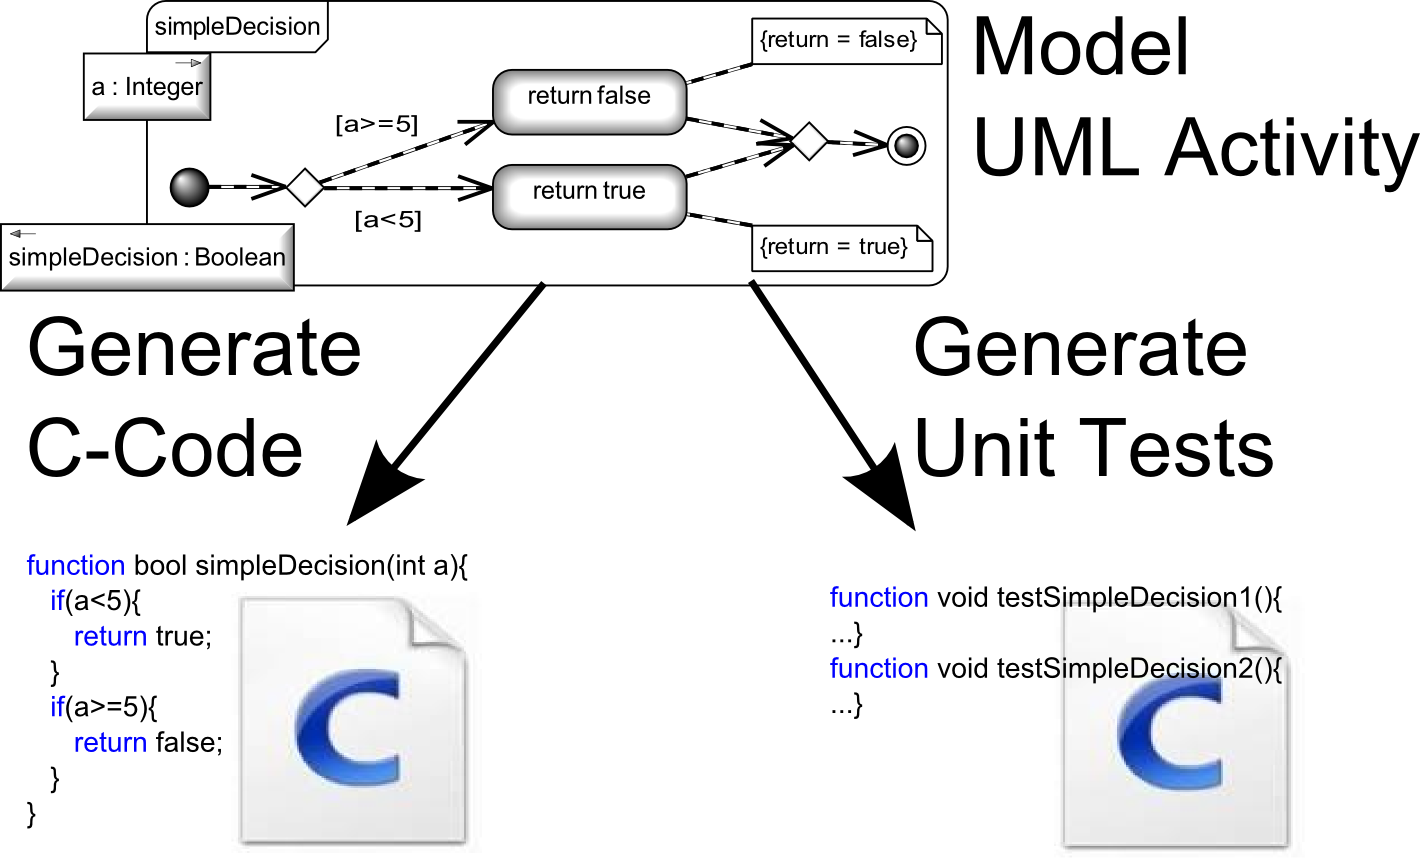
\includegraphics[width=0.7\textwidth]{./pics/Activity2Code+Tests.png}
\caption{Example of an activity diagram and the generated C-Code and corresponding Unit Tests}
\end{figure}
At Airbus Buxtehude Model-Based Engineering shall soon replace the traditional requirement-driven engineering approach. There are some benefits that we hope to be able to realize with Model-Based Engineering. One benefit is the automatic generation of source code from the model. Another way to profit from Model-Based Engineering is to use the specification as a test model from which all Unit Test code for the software implementation could be deduced. In figure\ref{fig:Act2Code+Tests} we are visualizing the idea of using one activity diagram to generate implementation code and unit test code from it.\\
For modelling behaviour and control flow of C functions UML activities will be used. The company Atego\textsuperscript{\textregistered} already built a proprietary code generator for Airbus Buxtehude, which generates a folder structure, C source code files, and C header files from a UML model and fills function bodies with code generated from UML activities. The fact that the code is generated does not make it fault free. We still need to validate the generated code by unit tests. The task in this thesis is to demonstrate how engineers can be supported at building the Unit Tests for the generated code. We decided to automate the generation of C++ Unit Tests from UML activities just as the generation of the C implementation was automated by the code generator from Atego\textsuperscript{\textregistered}.\\
%\subsection{Independence of Souce code and Testmodel}
One should not generate both the source code and the unit test from the same model. The implementation model needs to be independent from the test model, otherwise one would end up testing the implementation against itself. That would not be meaningful. %We need independence between the implementation and the corresponding unit tests.
%Writing the complete unit test code by hand is cumbersome. 
Generating Unit Tests from a complete new model that is build independently from the model used for code generation imposes a lot of work. The decision was to share the structure of the activity between code generation and test generation. While the code generation uses procedural C code snippets that are embedded in the model the test generation only relies on embedded declarative OCL constraints. By using two different programming paradigms as input for code generation and test generation we assume the generated C-implementation to be independent from the generated Unit Tests.


\section{Idea of this Thesis}
This thesis focuses on generating unit tests from UML activities with embedded OCL constraints. Our approach is based on mathematical programming to make the test model executable and find useful test data to test the implementation. We are putting some emphasis on mixed integer non linear arithmetic constraints and will evaluate the limits of state of the art mathematical solver implementations.
\subsection{Model Transformations}
A UML activity diagram will be transformed into a rigorous, executable, mathematical program. We decided to use model transformations to do this transformation stepwise. In section (\ref{sec:Normalisation}) we will transform the UML and OCL input into an intermediate representation. During this transformation we can check some design rules and ensure some properties of the intermediate representation that are necessary in subsequent steps. From this intermediate representation we perform a model to text transformation to a mathematical programming language (\ref{sec:atcg2Ampl}).
\subsection{Mathematical Programming}
As mathematical modelling language AMPL will be used. The activity will be represented by arrays of variables and indexed collections of arithmetic constraints. In a data section for the model we can specify which control flow path within the activity we are interested in. When building the mathematical program from the activity care needs to be taken that the semantic of the resulting model corresponds with the semantic the modeller originally had in mind.
\subsection{State-of-the-art Constraint Solver Implementations} 
A great advantage of a commonly used mathematical programming language is that there are industry strength solvers available. By running a state-of-the-art solver the constraint system will be solved for any possible path in the activity. This results in possible input arguments for the C function implementing the activity. Also all expected return values as well as values for class properties before and after the execution of the activity will be computed. Depending on the problem formulation a suitable solver needs to be selected. Not every solver can solve every mathematical program, and not every mathematical program is an instance of an easy to solve problem. An overview over problems that are considered throughout this thesis can be found in (\ref{sec:Maths}).
\subsection{Results}
One result of this thesis is an Eclipse plug-in automatically generating unit tests for activities. The plug-in comes with a set of test models. Each example is an instance of another mathematical problem and thus needs another solver to be solved successfully. Moreover we performed an industrial case study using a model of the PAX-Call system in an Airbus. We added the missing OCL constraints and successfully generated test cases for on of the activities within the model.

%To be precice at airbus the decicion was to use UML Activities for modelling behavior and controll flow of C functions for embedded Systems. 
%Basically we want to harvest the benefits from Model Based Engineering by building tool support to generate a test suite for a C function. 
%The generated Test Suite should of course be complete according to some coverage criteria to be selected by the user. 
%And it needs to integrate with the currently used Modelling tools. 
%There is no use in having a Tool working with models when you can not use the models from your standard modelling environment but have to build new models. 

%\subsection{Behavioural Modelling}
%\subsection{Generating Unit Tests from Behavioural Model}
%Explain Model Based engineering at Airbus Buxtehude with Component structure of the software and code generation as well as Test generation from a Model.
%Give the short overview over the complete thesis

\section{Outline}
The rest of this thesis is organized in 3 chapters. In the \nameref{chap:preliminaries} we will explain the assumed input language (\ref{sec:UML}), give an overview over the theory of mathematical programming and constraint programming (\ref{sec:Maths}), refer to some related work being done by other scientists (\ref{sec:RelatedWork}), and explain the mathematical programming language AMPL which we are going to use to make our models executable.\\
In the chapter \nameref{chap:testgeneration} we first give a short overview over the overall algorithm (\ref{sec:testgenerationOverview}) and then explain the fife subsequent steps of the algorithm. Each of them can be viewed as model-to-model, model-to-text, or text-to-model transformation (\ref{sec:Normalisation}), (\ref{sec:atcg2Ampl}), (\ref{sec:pathsearch}), (\ref{sec:testgenerationSolving}) and (\ref{sec:testgenerationUnitTestSynthesis}. The last section (\ref{sec:testgenerationImplementation} is about the implementation of the presented algorithm in an Eclipse plug-in.\\
The chapter \nameref{chap:evaluation} presents the example collection (\ref{sec:evaluationAcademicModels} that has been tested with the implemented eclipse plug-in and elaborates the strengths of different solvers. Also the case study (\ref{sec:evaluationCaseStudy} can be found in the \ref{chap:evaluation}rd chapter. Finally we will also summarize a few problems that could not be solved within this thesis (\ref{sec:evaluationLimitations}).